\documentclass[10pt]{beamer}
\mode<presentation>
{
	%\usetheme{Berkeley}
     %\usetheme{Warsaw}
      \usetheme{Singapore}
	%\usetheme{Goettingen}
	%\usetheme{Dresden}
	%\usetheme{Boadilla}
	\setbeamercovered{transparent}
	% or whatever (possibly just delete it)
}

\usepackage{caption}
\usepackage[font={small,it}]{caption}
\usepackage[justification=centering]{caption}
\usepackage[english]{babel}
% or whatever
\usepackage{tikz,dsfont}
\usepackage{inputenc}
\usepackage{times}
\usepackage[T1]{fontenc}
% Or whatever. Note that the encoding and the font should match. If T1
% does not look nice, try deleting the line with the fontenc.

\usepackage{amsmath, amssymb ,dsfont, graphicx, hyperref}
\usepackage{epsfig}
\usepackage{changepage}
\usepackage{listings}
\usepackage{xcolor}

\lstset{
	basicstyle=\ttfamily\scriptsize,
	breaklines=true,
	frame=single,
	backgroundcolor=\color{gray!10},
	keywordstyle=\color{blue},
	commentstyle=\color{green!50!black},
	stringstyle=\color{red!70!black},
	language=Python
}

\renewcommand{\pmod}[1]{\,(\textup{mod}\,#1)}
\numberwithin{equation}{section}
\newtheorem{conjecture}[theorem]{Conjecture}
\newtheorem{proposition}[theorem]{Proposition}
%\newtheorem{definition}[theorem]{Definition}
%\newtheorem{example}[]{Example}

\title[passagemath]
{Contributing to passagemath}

\subtitle
{Fixing inline plots in Colab}

\author[]
{
	Your Name
}


\institute[]
{

		\centering
		
\includegraphics[width=0.2\textwidth]{math_logo.png}

	
}


\date[]
{\scriptsize Davis Math Lab Presentation\\ May 20--21, 2026}

\subject{Talks}




\AtBeginSubsection[]
{
	\begin{frame}<beamer>{}
		\tableofcontents[currentsection,currentsubsection]
	\end{frame}
}

\begin{document}
	\maketitle

\section{The problem}
	\begin{frame}{What is passagemath?}
		\begin{itemize}
			\item Free, open-source software for doing math
			\item Plotting, linear algebra, graph theory, number theory, optimization, \ldots
			\item Community-maintained fork of SageMath
			\item Designed to be \textbf{modular}: install only the pieces you need
		\end{itemize}
	\end{frame}

	\begin{frame}{The problem: plots didn't render in Colab}
		When you tried to plot something in Colab, you'd just see text:
		\vspace{0.5em}
		\begin{center}
		\texttt{Graphics object consisting of 1 graphics primitive}
		\end{center}
		\vspace{0.5em}
		Colab needs to be told \emph{how} to turn a plot into an image, and passagemath wasn't telling it.
	\end{frame}

	\begin{frame}[fragile]{The workaround}
		Users had to paste this at the top of every notebook:
		\begin{lstlisting}
from io import BytesIO
from matplotlib.backends.backend_agg import FigureCanvasAgg
from sage.plot.graphics import Graphics

def _graphics_repr_png(self):
    figure = self.matplotlib()
    figure.set_canvas(FigureCanvasAgg(figure))
    buf = BytesIO()
    figure.savefig(buf, format='png')
    return buf.getvalue()

Graphics._repr_png_ = _graphics_repr_png
		\end{lstlisting}
		Works, but you have to remember it every time.
	\end{frame}

\section{Progress Report}
	\begin{frame}{The fix: PR \#2351}
		Moved the workaround into passagemath itself, so the library knows how to draw its own plots.
		\vspace{1em}
		\begin{itemize}
			\item Merged into version 10.8.5
			\item No more boilerplate at the top of every notebook
			\item \texttt{plot()} just works
		\end{itemize}
	\end{frame}

	\begin{frame}[fragile]{Demo 1: plotting a function}
		\begin{columns}
			\begin{column}{0.45\textwidth}
				\begin{lstlisting}
from sage.plot.plot import plot
import math
plot(math.sin, 0, 6)
				\end{lstlisting}
			\end{column}
			\begin{column}{0.55\textwidth}
				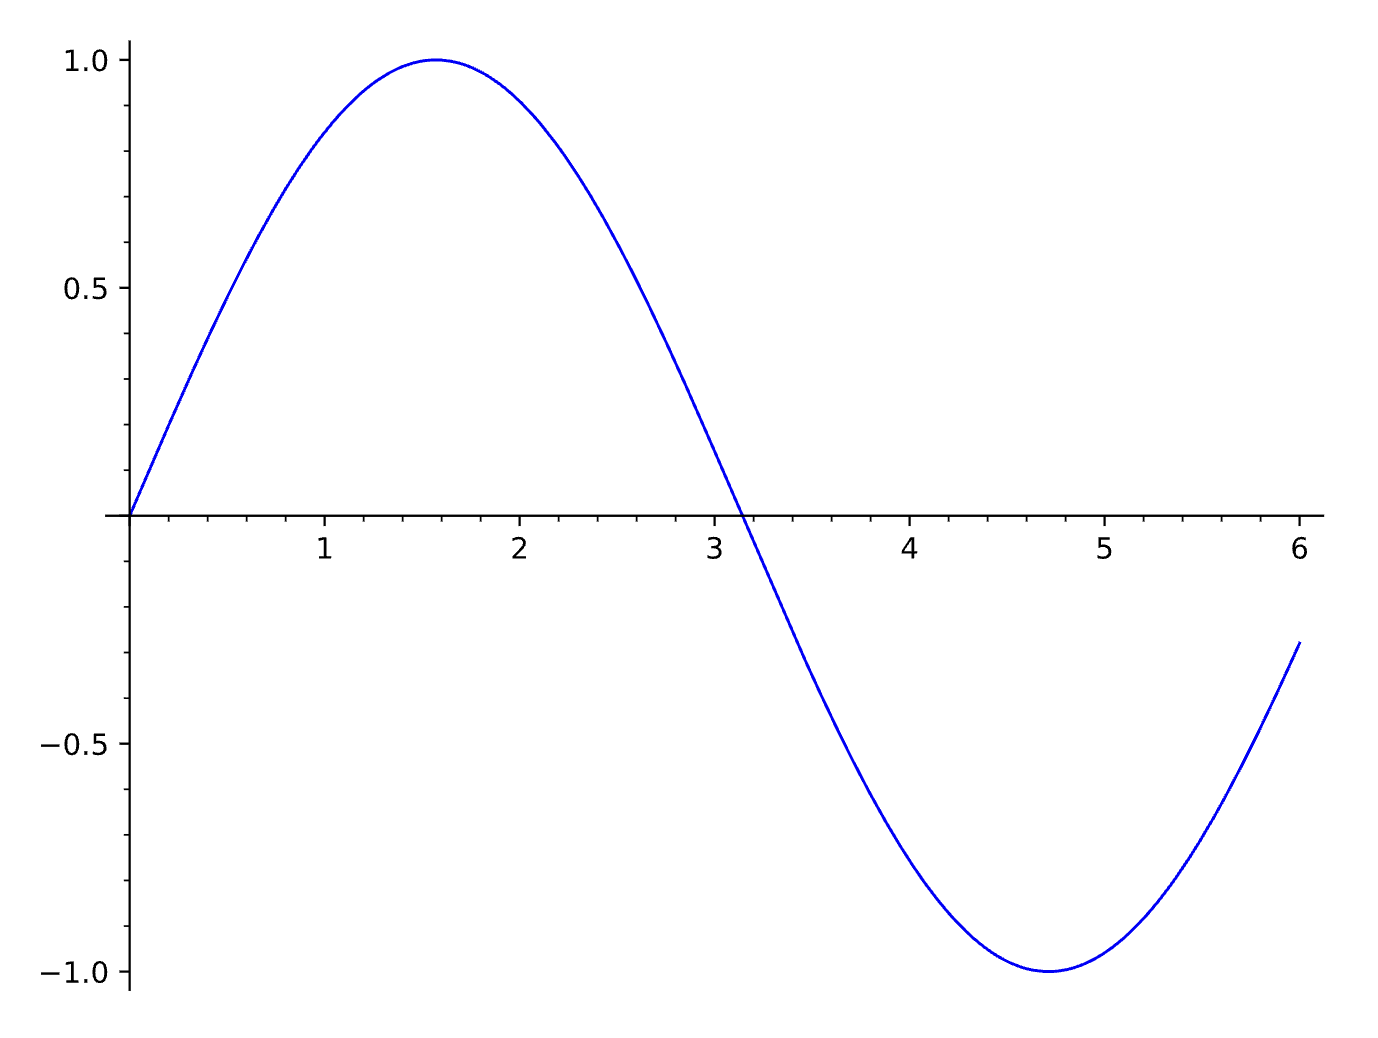
\includegraphics[width=\textwidth]{screenshot_sin.png}
			\end{column}
		\end{columns}
	\end{frame}

	\begin{frame}[fragile]{Demo 2: linear programming}
		\begin{columns}
			\begin{column}{0.45\textwidth}
				\begin{lstlisting}
A = ([3, 2], [1, 2])
b = (12, 8)
c = (2, 3)
P = InteractiveLPProblem(
    A, b, c, ["x1", "x2"],
    variable_type=">=")
P.plot()
				\end{lstlisting}
				\vspace{0.5em}
				\scriptsize The shaded region is the feasible set; the optimum sits at a corner.
			\end{column}
			\begin{column}{0.55\textwidth}
				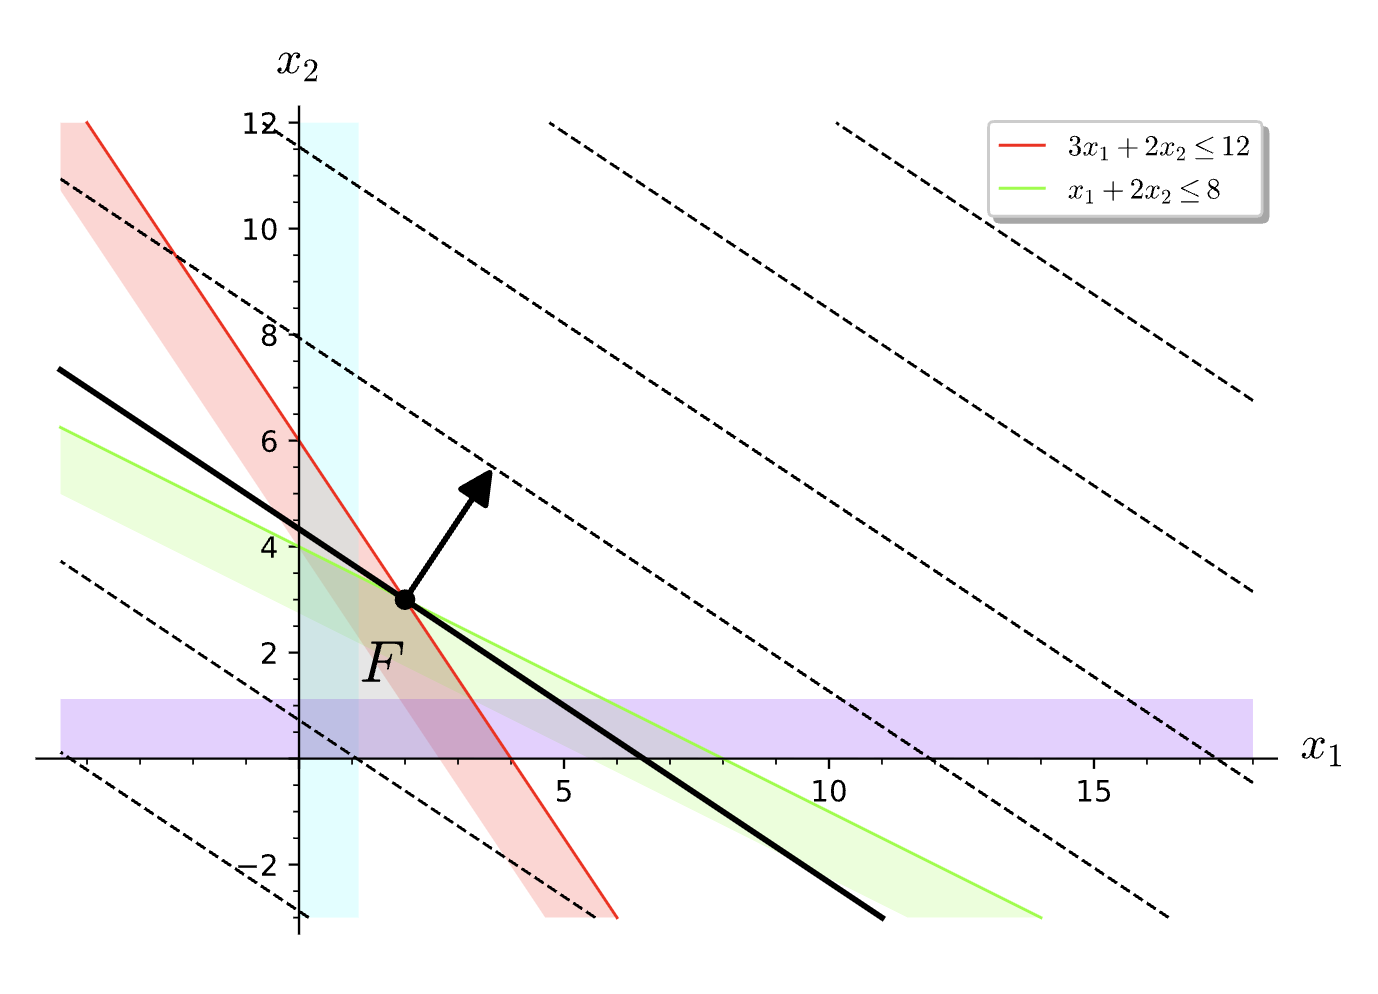
\includegraphics[width=\textwidth]{screenshot_lp.png}
			\end{column}
		\end{columns}
	\end{frame}

	\begin{frame}[fragile]{Demo 3: graph theory}
		\begin{columns}
			\begin{column}{0.45\textwidth}
				\begin{lstlisting}
from sage.graphs.generators.chessboard \
    import QueenGraph
G = QueenGraph([3, 3])
G.plot()
				\end{lstlisting}
				\vspace{0.5em}
				\scriptsize Every square a queen can reach from every other square on a $3 \times 3$ board.
			\end{column}
			\begin{column}{0.55\textwidth}
				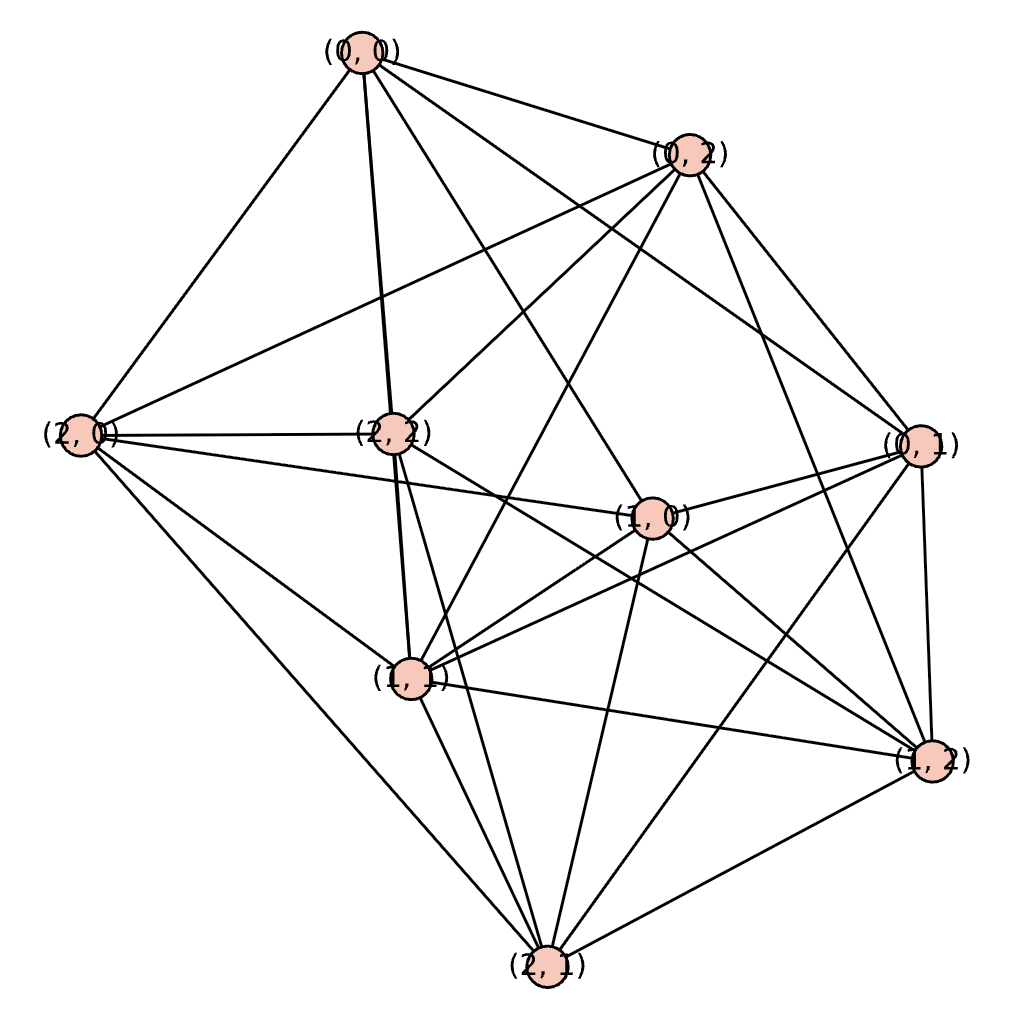
\includegraphics[width=\textwidth]{screenshot_queen.png}
			\end{column}
		\end{columns}
	\end{frame}

\section{Future Plans}
	\begin{frame}{What's next}
		\begin{itemize}
			\item Continue contributing bug fixes and features
			\item Help make passagemath the default way to use Sage on Colab
			\item Improve documentation and onboarding for new contributors
		\end{itemize}
	\end{frame}

\section{Other Activities}
	\begin{frame}{Other activities}
		\begin{itemize}
			\item (anything else you've done with the math lab)
		\end{itemize}
	\end{frame}

\end{document}
